\chapter{Fundamentação Teórica}
Este capítulo apresenta os conceitos básicos sobre som, quais as representações e estruturas do áudio digital, o que é informação musical e como é feito o seu armazenamento em bancos de dados, por fim, o tema recuperação da informação musical.

%CONCEITOS BÁSICOS SOBRE SOM%
\section{Conceitos Básicos sobre Som} \label{conceitoSom}
Nós ouvimos uma variedade de sons à todo momento e vivemos toda a nossa vida rodeados por eles. Sons de portas abrindo e fechando, dos passos, do ruído dos motores dos automóveis, da chuva e da música. O som não é algo que podemos ver com nossos olhos \cite{miletto2004}. Então, o que é o som? 
Um som é gerado por algum objeto vibratório, em uma repetição periódica de deformações e restaurações \cite{muller2007}. Estas vibrações produzem mudanças de pressão do ar, resultando em regiões locais de ar que são mais densas e outras que são rarefeitas, ocorrendo sucessivamente uma depois da outra e expandindo-se. Estas são chamadas condensações e rarefações. O processo é similar ao que conhecemos quando jogamos uma pedra dentro d’água, a qual produz ondas circulares em sua superfície. Estas ondas de condensações e rarefações são propagadas para dentro do ouvido humano e irão vibrar o tímpano. As vibrações do tímpano são captadas pelas nossas terminações nervosas, de maneira que nós as escutamos como sons. Se os corpos que vibram são diferentes, também será diferente a classe de vibração que produzem. Isto significa que escutamos distintas classes de sons.
Outra forma, é através de aparelhos chamados \textit{tradutores}, por exemplo, um microfone, que converte as vibrações em corrente elétrica equivalente ao sinal sonoro \cite{paulozuben2004}.

Se essa pressão do ar varia de acordo com um padrão repetitivo, dizemos que o som tem uma forma de onda periódica. Se não há um padrão perceptível no som, este é chamado de ruído. Ainda, quando as variações na pressão do ar são representadas de forma gráfica, elas podem ser interpretadas como “formas de onda”. Na Figura \ref{fig:ondaSenoidal}, a representação gráfica de um som mostra as mudanças na pressão do ar conforme a passagem do tempo. Lendo-se o gráfico da esquerda para a direita, quando a linha curva está próxima da parte inferior do gráfico então a pressão do ar é mais baixa e quando a curva está próxima do topo do gráfico, a pressão do ar aumentou \cite{miletto2004}.

\begin{figure}[!htb]
   \centering
   \caption{Representação gráfica, no domínio temporal, de uma forma de onda senoidal}\label{fig:ondaSenoidal} 
   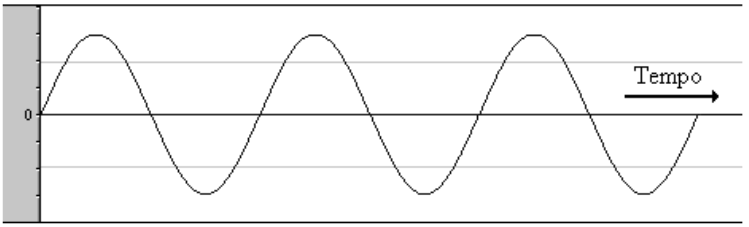
\includegraphics[scale=0.50]{figuras/ondaSenoidal.png}
   \\Fonte: \cite{miletto2004}.
\end{figure}

Segundo \citeonline{miletto2004}, os quatro elementos básicos do som são:
\begin{enumerate}
\item \textit{Altura tonal}: É a “altura” de um som, ou seja, se é alto ou baixo, agudo ou grave. A repetição de uma onda periódica é chamada de ciclo. O número de ciclos dentro do intervalo de um segundo é chamado freqüência, medida em hertz (Hz), que é então a recíproca do período. Quanto maior o valor em hertz, mais agudo é o som. Dobrando a freqüência de um som, este é elevado em uma oitava. Então, é possível dizer que a freqüência e a altura tonal estão relacionadas logaritmicamente.

\item \textit{Volume}: A mudança no volume de um som pode ser vista como uma diferença na altura das ondas. A altura de uma onda chama-se “amplitude”. Quanto maior a amplitude, mais forte é o som. Portanto, o volume de um som é determinado pela amplitude.

\item \textit{Timbre}: É o que diferencia dois sons de mesma frequência. De um modo geral, formas de ondas arredondadas produzem um timbre mais suave enquanto que as formas de ondas ponteagudas dão um timbre mais penetrante e estridente.

A Figura \ref{fig:ondaTimbre} mostra três formas de onda básicas, seus timbres característicos e os instrumentos que se assemelham a cada caso.

\begin{figure}[!htb]
   \centering
   \caption{Formas de onda simples e seus timbres}\label{fig:ondaTimbre} 
   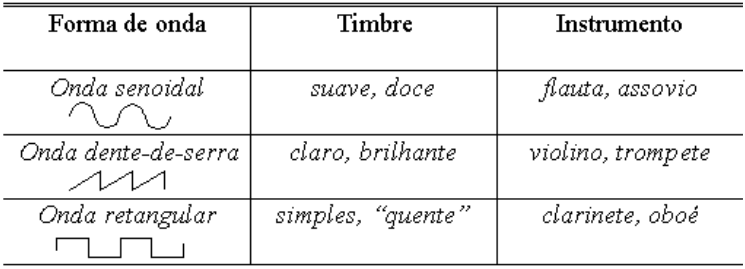
\includegraphics[scale=0.50]{figuras/ondaTimbre.png}
   \\Fonte: \cite{miletto2004}.
\end{figure}

\item \textit{Envolvente da Onda}: É a variação da altura tonal, do volume e do timbre em um transcurso de tempo que vai desde o começo do som até um ponto do tempo onde ele desaparece completamente. Estas mudanças no tempo são o que determina o timbre característico de um objeto, além do seu espectro harmônico.
\end{enumerate}

Os sons com vibrações regulares - que são os harmônicos e a fundamental \footnote{Por definição, o primeiro harmônico corresponde à freqüência fundamental, o segundo harmônico ao primeiro harmônico e assim por diante \cite{muller2007}.} - são considerados sons musicais, enquanto os sons causados por vibrações irregulares - que não são harmônicos - cuja altura tonal não pode, portanto, ser medida, são chamados sons não-musicais. A maioria dos sons usados na música são, por pressuposto, sons musicais.

%REPRESENTAÇÃO DO AUDIO DIGITAL%
\section{Representação do Áudio Digital} \label{formatos}

Como comentado anteriormente, o som é a variação da pressão do ar. Sendo assim, a forma de produzir um determinado som depende da maneira como a pressão do ar varia. Para \citeonline{miletto2004}, o processo de representar numericamente o som é chamado de \textit{digitalização}, ou seja, é representar uma onda sonora (áudio analógico) em código binário (áudio digital). 

A digitalização das formas de onda consiste em três etapas, realizadas por um circuito chamado \textit{conversor analógico/digital} (A/D) \cite{paulozuben2004}: \textit{amostragem}, \textit{quantização} e \textit{codificação}. Na primeira etapa, a forma de onda é lida ou amostrada em curtos intervalos de tempo uniformes (\textit{samples}). Então, na segunda etapa, o valor da forma de onda em cada ponto amostrado é restrito ou quantificado para um conjunto discreto de valores. Por fim, na terceira etapa é feita a codificação, traduzindo os valores para código binário. É uma transformação com perdas, no sentido de que se perde informação neste processo. (ver Figura \ref{fig:ondaAnalog}).

\begin{figure}[!htb]
   \centering
   \caption{Forma de onda analógica (curva preta) e representação digitalizada (as amostras digitalizadas são indicados pelas caixas cinzentas). Neste exemplo, a forma de onda é amostrada em 24 pontos e a quantização dos valores emprega um esquema de codificação de 4 bits (16 valores possíveis)}\label{fig:ondaAnalog} 
   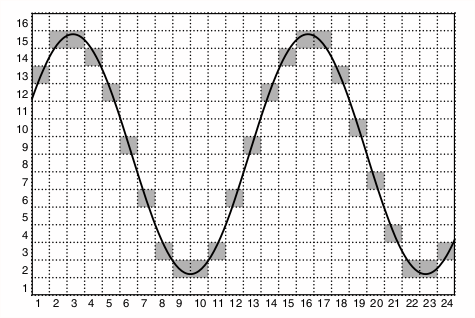
\includegraphics[scale=0.8]{figuras/ondaAnalog.png}
   \\Fonte: \cite{muller2007}.
\end{figure}

Para podermos ouvir as informações transformadas em linguagem digital pelo conversor A/D, é preciso realizar o processo inverso, utilizando um \textit{conversor digital/analógico} (D/A) \cite{paulozuben2004}.

Inicialmente, armazenar dados de áudio em formato analógico discretizado consome muito espaço \cite{juliana2004}, e como solução foi adotada a codificação MIDI (\textit{Musical Instrument Digital Interface}). Essa codificação é uma representação numérica do som, sendo usada atualmente como o formato de intercâmbio de música digital simbólico mais comum para possibilitar a transferência de informações entre instrumentos musicais e computadores \cite{muller2007}. O tamanho desses arquivos tende a ser bem reduzido, já que a codificação de eventos musicais pode ser bem compacta.

Embora isso seja satisfatório em algumas situações, arquivos MIDI (extensão .mid ou .smf) basicamente codificam apenas instruções referentes a notas e durações e não a informação sonora propriamente dita \cite{fernando&kon1998}. Ou seja, seu código são instruções para um sintetizador correspondentes a eventos musicais como soar uma nota, silenciar uma nota, mudar o andamento ou o tom da música, etc. O sintetizador, por sua vez, interpreta este código e o executa, podendo usar vários timbres de instrumentos simultaneamente \cite{miletto2004}, e por isso, o resultado sonoro é totalmente dependente da qualidade e das possibilidades oferecidas por esse aparelho \cite{fernando&kon1998}.

Com o mesmo objetivo, os formatos \textit{Wave}, da Microsoft (extensão .wav) e \textit{AIFF}, da Apple (extensão .aiff ou .aif) são do tipo áudio digitalizado sem compressão. Baseiam-se na codificação PCM (\textit{Pulse Code Modulation}), onde a própria onda sonora é representada como uma sucessão de números correspondentes às amplitudes do sinal medidas a uma freqüência constante. Ou seja, armazenam dados de um processo de digitalização simples. A diferença para com o formato MIDI, é que esse tipo de codificação origina um grande volume de dados e exige muito espaço para armazenamento e sua única vantagem é a reprodução fiel do áudio se o arquivo for gravado com qualidade de CD \cite{miletto2004}.

Outro recurso é a compressão de dados, que é feita através de programas ou \textit{hardware} específicos que compactam os arquivos de áudio, reduzindo o seu tamanho, antes de serem enviados. Ao chegar ao seu destino, esses arquivos são descompactados e, em seguida, tocados. Entretanto, compressão, nesse contexto, é sinônimo de perda de qualidade: quanto maior a compressão, maior também a quantidade de informação que se perde \cite{fernando&kon1998}. Apesar disso, certos padrões de compressão já permitem a transmissão de arquivos de áudio de boa qualidade em tempo real, o que resulta na existência de uma quantidade equivalente de formatos de arquivo para a compressão do som digitalizado \cite{miletto2004}.

Segundo \citeonline{miletto2004}, os formatos de arquivo mais utilizados para a compressão de som são:

\begin{itemize}
    \item MPEG Layer 3 (extensão .mp3);
    \item Advanced Audio Coding (extensão .aac);
    \item Windows Media Audio, da Microsoft (extensão .wma);
    \item Real Audio, da RealNetworks (extensão .ra);
    \item Sun Audio, da Sun (extensão .au).
\end{itemize}

Em paralelo, quando o áudio foi do analógico para o digital, tornou-se possível codificar arquivos de áudio com mais informação do que apenas o nome do arquivo - os \textit{metadados}.

Os metadados podem ser usados para nomear, descrever, catalogar e indicar os direitos de autor de um arquivo de áudio digital. Como diferentes formatos de áudio digitais foram desenvolvidos, foi acordado que um local padronizado e específico, seria reservado dentro dos arquivos digitais onde estas informações pudessem ser armazenadas.

Existem padrões diferentes de metadados para finalidades distintas de informações. Para o áudio digital, o padrão mais utilizado é o ID3 (abreviação de \textit{Identify a MP3}). 

O ID3 começou a ser idealizado a partir de 1996 por Eric Kemp. Em sua primeira versão o ID3 limitava-se apenas a 128 B \abreviatura{B}{Byte} de informação e essas informações também eram limitadas quanto ao número de caracteres. Já na segunda versão, idealizada a partir de 1998, o padrão tornou-se mais completo, permitindo que mais informações pudessem ser adicionadas já que o limite passa a ser de 256 MB \abreviatura{MB}{Megabyte} \cite{ferreira2015}.

Na Tabela \ref{tab:diferencasId3} é possível verificar as diferenças entre as versões do ID3.

\begin{table}[ht]
    \centering
    \caption{Diferenças entre as versões ID3}
    \begin{tabular}{|p{4cm}|p{4cm}|}
    \hline
        ID3v1 & ID3v2 \\
    \hline
        128 bytes & 256 mb \\
    \hline
        Título & Título \\
    \hline
        Artista & Artista \\
    \hline
        Álbum & Álbum \\
    \hline
        Ano & Ano \\
    \hline
        Comentário & Comentário \\
    \hline
        Gênero & Gênero \\
    \hline
         & Compositores \\
    \hline
         & Letra da música \\
    \hline
         & Capa do álbum \\
    \hline
    \end{tabular}
    \label{tab:diferencasId3}
    \\Fonte: Elaborado pela autora
\end{table}

Existem diversos \textit{softwares} que editam as \textit{tags} ID3, porém, na maioria das vezes esses \textit{softwares} disponíveis não permitem a edição completa dos dados de descrição do áudio.

Desta forma, podemos afirmar que um arquivo de áudio digital é composto por metadados e som digitalizado, sendo assim, um dado musical.

%INFORMAÇÃO MUSICAL%
\section{Informação Musical}
Para \citeonline{setzer2001}, dado é uma sequencia de números, portanto, um texto, fotos, figuras, sons gravados e animação são dados, pois todos podem ser amostrados, quantificados e codificados. Um dado é necessariamente uma entidade matemática e, desta forma, é puramente sintático. Isto significa que os dados podem ser totalmente descritos através de representações formais, estruturais e obviamente ser armazenados em um computador e processados por ele.

O dado é a representação física de um evento no tempo e espaço que não agrega fundamento, não podendo ser possível entender o que ele representa ou para que ele existe, se somente for disponibilizado para alguém ou para o tempo e espaço, por alguém ou por um evento, não é possível saber o que ele significa ou o que ele representa, podendo representar qualquer coisa ou não representar nada, porém, ao incluir um “significado” no dado e gerar sentido para quem o ouve e ficando claro ou não a que se refere, é gerada a informação \cite{rafael2013}.

O autor \citeonline{setzer2001} expõe que a informação é uma abstração informal (isto é, não pode ser formalizada através de uma teoria lógica ou matemática) que está na mente de alguém, representando algo significativo para essa pessoa. A frase “Paris é uma cidade fascinante” é um exemplo de informação desde que seja lida ou ouvida por alguém, desde que "Paris"\ signifique para essa pessoa a capital da França (supondo-se que o autor da frase queria referir-se a essa cidade) e "fascinante"\ tenha a qualidade usual e intuitiva associada com essa palavra.

A informação pode ser armazenada em um computador, ou melhor, a sua representação em forma de dados e não a informação propriamente dita. Essa representação pode ser transformada pela máquina, como na formatação de um texto, mas não pode mudar o significado, já que ele depende de uma pessoa que possui a informação. Os dados são sempre incorporados por alguém como informação, porque os seres humanos buscam constantemente por significação e entendimento.

A partir daí, a autora \citeonline{barros2012} expõe que um dado musical é resultado de um processo de significação social. Assim, a música é uma expressão humana construída socialmente e objetivada por meio de sua comunicação oral, registro sonoro ou representação gráfica.

Para \citeonline{almeida2007}, a obra musical é efêmera e abstrata, pois só se concretiza no momento de cada interpretação, na execução da música. \citeonline{berger&luckmann2014} afirmam que:

\begin{citacao}
A expressividade humana é capaz de objetivações, isto é, manifesta-se em produtos da atividade humana que estão ao dispor tanto dos produtores quanto dos outros homens, como elementos que são de um mundo comum \cite{berger&luckmann2014}.
\end{citacao}

Para \citeonline{angeles2010,pinheiro&loureito1995}, a informação é o que se acrescenta a uma representação. Segundo os autores, recebemos informação se o que conhecemos é alterado. Informação é o que logicamente justifica alteração ou reforço de uma representação ou de um estado de coisas. As representações podem ser explícitas (como em um mapa ou em uma proposição), ou podem estar implícitas no estado de atividade dirigida do receptor.

A informação musical apresenta determinadas especificidades de comportamento na sua produção, objetivação e uso, pois a manifestação da música apresenta-se carregada de características próprias. \citeonline{michels1992} explica que a música contém dois elementos: o \textit{material acústico} e a \textit{ideia intelectual}, sendo que tais elementos não se encontram justapostos, mas sim se combinam para formar uma imagem unitária. Portanto, a compreensão completa da música está diretamente ligada com o reconhecimento do contexto histórico e social de sua origem, com a interpretação pessoal e individual do ouvinte, e com os aspectos sonoros que a constituem. Dessa forma, a música tem diferentes significações para cada indivíduo.

\citeonline{lima&santini2006} afirmam que:

\begin{citacao}
A música é um produto social e simbólico de grande importância nas diferentes formações culturais, principalmente se considerarmos a sua capacidade de criar vínculos afetivos e cognitivos entre as pessoas \cite{lima&santini2006}.
\end{citacao}

A compreensão da música como informação é ainda bastante recente. O estudo mais significativo e considerado, dentro da literatura especializada, como pioneiro na conceituação e estudo da música como fonte de informação é o de Alexander McLane. Em 1996, o autor publicou em um capítulo do \textit{ARIST} (\textit{Annual Review of Information Science and Technology}) o artigo intitulado \textit{Music as Information}, onde formaliza a música como informação.

%ARMAZENAMENTO DA INFORMAÇÃO MUSICAL%
\section{Armazenamento da Informação Musical}

Até o surgimento dos inventos tecnológicos, a música era um meio de comunicação exclusivamente presencial. Apesar das formas de registros, a exemplo das partituras, possibilitarem a execução de uma obra em diferentes momentos e lugares, a reprodução do que ali estava representando nunca seria a mesma. Com o decorrer do tempo,  as técnicas e invenções aplicadas ao processo de gravação do som foram surgindo e se aperfeiçoando, resultando em aparelhos reprodutores e suportes cada vez mais versáteis e manipuláveis \cite{daquino2012}. Especialmente após o desenvolvimento das coleções em rede na \textit{Web}, com formatos de arquivos compactados e custos decrescentes de armazenamento de arquivos na forma digital, a música se tornou um objeto de consumo universal e extremamente acessível \cite{gomes2015}.

Os dispositivos de armazenamento musical são divididos em dois grandes grupos: \textit{analógicos} e \textit{digitais} \cite{andrade&crispim2008}. Os analógicos são antecessores dos digitais e foram o meio tecnológico dominante em boa parte do século XX \cite{paulozuben2004}. O primeiro invento significativo foi o fonógrafo, patenteado por Thomas Edison em 1877. Dez anos mais tarde, em 1887, surgiu o gramofone, tendo uma capacidade maior de armazenamento e reprodução das músicas \cite{marchi2005}. 

Dentre as invenções mais importantes para o armazenamento e a reprodução sonora analógica está o disco de vinil, lançado em 1948, comumente conhecido como LP\abreviatura{LP}{\textit{long-play}}. Era um disco com rotação por minuto mais demorada, o que permitia aumentar a capacidade de armazenamento da informação na superficie do vinil. Em seguida, entre as décadas de 60 e 70, com a evolução dos cartuchos 8-track (pioneiros em armazenar dados musicais em fitas magnéticas), o lançamento da fita cassete ou \textit{compact cassette} \cite{marchi2005}, era basicamente, dois carretéis, a fita magnética e todo o mecanismo de movimento da fita, alojados em uma caixa plástica \cite{andrade&crispim2008}.

No armazenamento analógico, as formas de onda dos sinais elétricos emitidos do aparelho eram registradas similarmente, isto é, de maneira análoga, pelas partículas magnéticas encontradas na fita. No momento da reprodução, os sinais magnéticos impressos na fita são interpretados analogamente como diferenças de voltagem, isto é, sinais elétricos. Como o nível do sinal elétrico era muito baixo, utilizava-se um amplificador para que a variação de voltagem estivesse suficiente para mover os cones dos alto-falantes. Dizemos que esse processo é uma gravação analógica, pois a forma de onda do sinal gravado é análoga à forma de onda do sinal original captado \cite{paulozuben2004}.

Porém, a partir da década de 80, com a intensificação do uso de \textit{hardwares} e \textit{softwares}, surge um dos primeiros meios de armazenamento digital: o CD (\textit{Compact-Disc}). Ele acabou por se tornar um dos meios de armazenamento de dados musicais mais populares das décadas seguintes. Além de quebrar paradigmas na época, o CD foi inspiração para o desenvolvimento de outros meios de armazenamento como os DVDs\abreviatura{DVD}{\textit{Digital Versatile Disc}} e os discos de Blu-ray \cite{marchi2005}.

Entretanto, surgiu a necessidade de disponibilizar informações no dispositivo de armazenamento. Na era analógica, esses recursos estavam associados à capa e/ou contracapa. Todavia, com a mudança do paradigma para digital, necessitou-se que essas informações pudessem ser disponibilizadas digitalmente, porém, o CD de áudio não inclui em sua estrutura, por exemplo, o nome do disco ou o nome de suas faixas. Sendo assim, surgiram as bases de dados de CDs, que visam prover informações dos mesmos quando esses são utilizados por sistemas de mídia modernos \cite{andrade&crispim2008}.

Com o surgimento dos arquivos digitais de áudio, as músicas se desvincularam do suporte físico (CD) e passaram a ser vistas isoladamente. Esses tipos de arquivos requerem um espaço consideravel para seu armazenamento (chegando a ocupar dezenas de megabytes em disco), o que propiciou o surgimento de um formato mais compacto: O MP3 (\textit{Moving Picture Experts Group-1 Layer 3}).

O grande desenvolvimento tecnológico das redes de compartilhamento de arquivos contribuiram para uma maior aceitação de formato de áudio MP3 \cite{andrade&crispim2008}, por ser facilmente transportado em qualquer bolso ou mochila e pela sua longa vida útil, além do aumento gradativo de armazenamento com o passar dos anos \cite{marchi2005}. Sua invenção, propiciou a popularização de eletrônicos com portas USB e o surgimento de cartões de memória \textit{microSD}, prometendo maior capacidade, durabilidade e clareza sonora \cite{marchi2005}.

Com a Internet, a música ultrapassa os limites físicos da mídia - mergulhando no universo digital - e passa a circular livremente pela rede mundial de computadores através do \textit{streaming}, que tomou forma no final da década de 80 e começou a se desenvolver na década de 90, com a evolução dos SGBDs (\textit{Sistemas de Gerenciamento de Banco de Dados}) e o surgimento dos BDOOs (\textit{Bancos de Dados Orientado a Objetos}) \cite{junior&segundo2008}, que possibilitaram o armazenamento de multimidias, assim como a popularização de aplicativos móveis, conhecidos normalmente por \textit{apps}, que oferecem mais de 30 milhões de música a seus usuários, por exemplo, "Spotify"\footnote{https://www.spotify.com/br/} e "Deezer"\footnote{https://www.deezer.com/br/}.

A evolução dos arquivos musicais não foi acompanhada de tentativas de inserção de informações elementares da música a esses arquivos. Há pouco tempo não existia um padrão para a representação dos metadados associados a esses arquivos \cite{andrade&crispim2008}, e a recuperação dessa informação só será bem sucedida se esses documentos multimídias puderem ser representados de acordo com as suas peculiaridades \cite{gomes2015}.

%RECUPERAÇÃO DA INFORMAÇÃO MUSICAL%
\section{Recuperação da Informação Musical}

A área de pesquisa denominada \textit{Music Information Retrieval} (MIR - \textit{Music Information Retrieval}) ou Recuperação da Informação Musical (RIM), tradução literal incorporada pela corrente da área no Brasil, é definida, de acordo com \citeonline{futrelle&downie2002}, como:

\begin{citacao}
[...] uma agenda de pesquisa que, de forma geral, pretende desenvolver formas de gestão de coleções de obras musicais para preservação, busca, acesso e outros usos \cite{futrelle&downie2002}.
\end{citacao}

A agenda de pesquisas sobre a RIM intensificou sua produção recentemente com a explosão do interesse em coleções em rede que contenham obras musicais na forma digital, possibilitadas pelo desenvolvimento das citadas técnicas de compressão de áudio. Os pesquisadores de RIM observam que a motivação maior para essa área de pesquisa é o grande volume de música digital disponível na Internet que, quanto mais cresce, menos possibilita sua recuperação eficiente, visto que estão apenas disponíveis aos montes, mas sem o tratamento adequado \cite{gomes2015}.

A área de RIM conta com profissionais das mais diversas áreas inclusas na questão do tratamento e recuperação da informação musical como apresentado na Tabela \ref{tab:comunidadeRim}, traduzida por \citeonline{santini&souza2007}

\begin{table}[ht]
    \centering
    \caption{Comunidades de RIM}
    \begin{tabular}{|p{4cm}|p{4cm}|p{4cm}|}
    \hline
        Comunidade & Tipo(s) de instituição & Área de pesquisa \\
    \hline
        Ciência da Computação, Recuperação da Informação & Acadêmica, Comercial & Representação, Indexação, Recuperação, Aprendizado de máquina, Design de interface de uso \\
    \hline
        Engenharia de áudio, Processamento de sinais digitais & Acadêmica, Comercial & Compressão, detecção de critério, Localização de tom, Aprendizado de máquina, Classificação, Análise musical \\
    \hline
        Musicologia, Teoria Musical & Acadêmica & Representação, Análise musical \\
    \hline
        Ciência da Informação, Biblioteconomia & Bibliotecas, Acadêmica & Representação, Metadados, Estudos de usuário, Classificação, Direitos de propriedade intelectual, Design de interface de uso \\
    \hline
        Ciência Cognitiva, Psicologia, Filosofia & Acadêmica & Representação, Percepção, Estudos de usuário, Ontologia \\
    \hline
        Direito & Governamental, Profissionais da lei, Acadêmica & Direitos de propriedade intelectual \\
    \hline
    \end{tabular}
    \label{tab:comunidadeRim}
    \\Fonte: \apud{santini&souza2007}{futrelle&downie2002}.
\end{table}

A origem de RIM não apresenta uma ação interdisciplinar, o que prejudica todo o seu processo de comunicação científica. Como pontua \citeonline{santini&souza2007}:

\begin{citacao}
(...) não há uma sociedade (inter)disciplinar de RIM; um periódico ou livro-texto fundador onde pessoas interessadas podem adquirir as bases teóricas e práticas de RIM. Com exceção de alguns pequenos encontros interdisciplinares, muitos pesquisadores estão apresentando seus resultados para membros das suas próprias disciplinas. A literatura de RIM é difícil de ser localizada, lida e estudada, o que dificulta construir e sustentar uma área de pesquisa respeitável e próspera \cite{santini&souza2007}.
\end{citacao}

A escassa produção científica a respeito do tema e as características impostas pelas músicas acarretam em certas dificuldades para sua representação.

Como elucidado no final da seção 2.1 deste capítulo, o ponto de partida para os estudos sobre a música como fonte de informação e tratamento, representação e recuperação foi dado em 1996 por Alexander McLane. Neste mesmo período já era possível identificar o desenvolvimento de tecnologias de compressão de arquivos digitais de música para transmissão na Internet e a popularização da Internet no mundo \cite{santini&souza2007}.

Em seu estudo, McLane direciona sua discussão para os grandes problemas relacionados à representação de documentos de música e à recuperação destes documentos. Ele analisa aspectos significantes da música – sua notação e seu som –, e propõe algumas ideias para sistemas de recuperação de música e formaliza a música como informação segundo três visões: \textit{visão subjetiva}, \textit{visão objetiva} e \textit{visão interpretativa}. Segundo o autor, as necessidades dos vários tipos de análises musicais são tão diversas que é preferível considerar três “visões” sobre a representação da obra musical.

Em resumo adaptado, \citeonline{santini&souza2007} apresenta as principais características das visões estabelecidas por \citeonline{mclane1996}.

\begin{itemize}
    \item A visão \textit{subjetiva} da informação musical se faz por meio do uso do esquema de notação para representação da informação musical. A subjetividade se dá porque a escolha de elementos de notação geralmente representa uma obra em “contexto-dependente”. Sendo assim, a decisão da notação pode incluir ou excluir aspectos particulares da obra.
    \item A visão \textit{objetiva} está vinculada a audição e ao momento da execução musical. Um som gravado pode ser identificado como visão objetiva da obra musical. A sonoridade se caracteriza como objetiva por não se configurar como uma representação, mas como a obra em sua essência. O som musical uma vez gravado torna-se fixo e não está mais sujeito a variações editoriais e de performance. Segundo McLane, esta visão pode ser considerada a mais completa representação da música, ao passo em que inclui as facetas tom, tempo, harmonia, editorial e timbre.
    \item A visão \textit{interpretativa} é realizada através da análise de alguns aspectos da obra, englobando informações que não são diretamente dependentes do documento. Entram nessa categoria classificações e esquemas analíticos que elucidam características como o gênero musical e avaliações críticas.
\end{itemize}

De acordo com \citeonline{cruz2014}:

\begin{citacao}
Dentre as visões propostas por \citeonline{mclane1996}, a interpretativa possui uma característica interessante porque permite a independência formal do documento musical em relação ao suporte que o contém, assim como foi possível na informação textual \cite{cruz2014}.
\end{citacao}

Segundo \citeonline{mclane1996,santini&souza2007}, a representação da informação musical pode abranger as três visões apresentadas dependendo das necessidades de informação da comunidade usuária. De acordo com tradução das autoras, a conclusão de McLane seria a de que:

\begin{citacao}
Ambas as escolhas sobre a visão da representação da música e o grau de complementação da representação de uma obra depende da necessidade de informação do usuário. A recuperação de informação é um processo interativo que depende do conhecimento do usuário e do nível de complexidade da informação desejada. No caso da necessidade da simples identificação de uma obra musical, onde a informação bibliográfica não é unicamente suficiente, pode-se limitar a uma visão subjetiva envolvendo um subconjunto relativamente pequeno de elementos notados de uma obra, frequentemente o tom inicial de uma frase melódica. A representação tonal pode ser de forma tal que provavelmente o usuário espera e está apto para formular a indagação usando a mesma terminologia, ou pelo menos uma que é traduzível na forma de representação \apud{santini&souza2007}{mclane1996}.
\end{citacao}

Sendo assim, percebe-se que a recuperação da informação da música depende tanto da complexidade e da forma como a informação é representada como do nível de conhecimento prévio do usuário. Para \citeonline{santini&souza2007}: “Quanto menor o conhecimento do usuário, maior a necessidade de diferentes formas de representação. Cada visão da representação da música, demonstrada por McLane, não é suficiente isoladamente para identificar uma obra.”.

Outro autor presente nos estudos relacionados à representação e recuperação de informação musical e um dos representantes da área de RIM é o professor J. Stephen Downie da Universidade de Illinois, nos Estados Unidos. Downie escreveu, em 2003, outro artigo tido como marco no estudo da informação musical, intitulado \textit{Music Information Retrieval} também em um capítulo do ARIST. No trabalho em questão, \citeonline{downie2003} examina a multidisciplinaridade da área de RIM, identifica e explica alguns problemas relacionados a questão da representação e recuperação da informação musical. Para isso \citeonline{downie2003} resume a questão em quatro grandes desafios a serem enfrentados pelos pesquisadores da área.

De acordo com \citeonline{downie2003} os quatro desafios seriam:

\begin{citacao}
    \begin{enumerate}
        \item Considerar permanentemente as diferentes formas de representação da música, o que caracteriza o \textit{desafio multirepresentacional}. O copyright faz parte deste desafio.
        \item Cada época histórica e cada formação cultural criam modos próprios e singulares de se expressar através da música. A música transcende as fronteiras culturais e temporais. A ampla variedade de expressões musicais coloca em evidência o \textit{desafio multicultural}.
        \item Compreender e responder às diferentes formas de interação individual com a música e com os sistemas de RIM constitui o \textit{desafio multiexperimental}.
        \item Maximizar os benefícios de ter uma comunidade multidisciplinar de pesquisadores, enquanto minimiza a desvantagem inerente, representa o \textit{desafio multidisciplinar}.
    \end{enumerate} 
\end{citacao}

O desafio multirepresentacional é dividido em sete facetas a serem consideradas na descrição da música e que representam a estrutura musical \cite{downie2003}: tonal, temporal, harmônica, de timbre, editorial, textual e faceta bibliográfica, sendo as quatro primeiras relativas a aspectos sonoros da música com formas gráficas de representação em figuras rítmicas ou notações musicais, enquanto que as três últimas são representadas na forma gráfica e dizem respeito às informações de produção, intérprete, compositor, copyright, data de produção e outras \cite{barros2012}.

Apesar de completas, a interação dessas facetas resulta em um complexo tratamento da informação musical, visto que cada faceta citada possui, por si só, uma complexidade inerente e sofre um tipo de representação enquanto produto. As autoras \citeonline{santini&souza2007} resumem a problemática multirepresentacional da seguinte forma:

\begin{citacao}
    A complexa interação entre as facetas da música - tonal, temporal, harmônica, de timbre, editorial, textual e bibliográfica – evidencia um dos principais problemas de RIM: o desafio multirepresentacional. A escolha da representação da música – se baseada em símbolos, áudio ou ambos – adiciona-se a diversas questões: como, por exemplo, cada escolha determina a tecnologia, a organização, a recuperação e a interface entre requisitos e capacidades dos sistemas \cite{santini&souza2007}.
\end{citacao}

Sendo assim, apesar de possuir as facetas estabelecidas por \cite{downie2003}, a estrutura da música incorpora elementos extras que nos permitem defini-la como um objeto informacional mais complexo. Para \citeonline{cruz2014} a estrutura musical:

\begin{citacao}
    [...] incorpora elementos adicionais que permitem defini-la como um objeto informacional musical mais amplo, dotado de conteúdo – atributos internos e metadados descritivos – e, de contexto – associações com outros objetos musicais e não musicais, e com situações ou eventos em que este objeto musical está inserido \cite{cruz2014}.
\end{citacao}

O segundo desafio (multicultural) nasce da condição inerente à música de ser uma objetivação de algo extremamente subjetivo: a \textit{expressão humana}. Sendo assim, sofre a interferência de uma grande variedade de fatores, da cultura vigente no momento da produção musical e da localização geográfica desta produção.

O desafio multiexperimental diz respeito à percepção da música como experiência individual ou coletiva capaz de causar diferentes reações em diferentes momentos e situações, de cada mente e humor individual. Neste caso, ouvir uma música gravada funciona como “ajudar a memória” que traz a tona experiências prazerosas ou dolorosas relacionadas a uma música em especial \cite{downie2003,santini&souza2007}. As variações de pessoa para pessoa na forma de apropriação, apreciação e nos tipos de experiências emocionais que a música evoca demonstram de maneira pragmática o desafio multiexperimental.

O quarto e último desafio estabelecido por \citeonline{downie2003} é o desafio multidisciplinar. Como citado anteriormente, a diversidade intelectual da comunidade de pesquisadores de RIM é, ao mesmo tempo, uma vantagem e uma adversidade. A heterogeneidade das visões de mundo das disciplinas apresenta um problema particular. Cada disciplina traz suas crenças, práticas, questões de pesquisa e paradigmas de avaliação \cite{downie2003}. De acordo com \citeonline{futrelle&downie2002}, não há uma aceitação comum dos objetivos, técnicas e resultados obtidos nas pesquisas referentes à informação musical.

Percebe-se, portanto, que, se por um lado, a ação multidisciplinar dos pesquisadores envolvidos com o tema possibilita o surgimento de diversos avanços tecnológicos e que a cada dia são divulgadas novas soluções para o tratamento de conteúdos musicais, com algoritmos mais sofisticados, novas formas de indexação de músicas, novos tipos de interfaces de áudio e novas formas de representação musical, em contrapartida, é notável a dificuldade de comunicação entre esses resultados. Nota-se ainda a dificuldade de identificação desses conteúdos musicais, porque a música é complexa e possui um leque de propriedades que possibilitam abordagens, às vezes, contraditórias \cite{cruz2014}.

A análise documental da informação musical para sua representação apresenta complexidades, pois exige diferentes técnicas de extração de informações para distintas formas de apresentação \cite{downie2003}.

%MÉTODOS E ALGORITMOS PARA RECUPERAÇÃO DA INFORMAÇÃO MUSICAL%
\subsection{Métodos e Algoritmos para Recuperação da Informação Musical}

Um dado multimídia geralmente é representado por um conjunto de características extraídas do conteúdo da música. Isto porque dados multimídia são basicamente arranjos multidimensionais de valores derivados de vários sensores, que é uma representação limitada para definir a semântica do dado. Neste sentido, dados complexos raramente são comparados diretamente. Em vez disso, o conteúdo do dado (ou uma faceta do conteúdo) é analisado por meio de algoritmos especializados de análise, extraindo um conjunto de características que descrevem numericamente o dado \cite{kaster2012}. Desta forma, as aplicações que lidam com dados complexos, como dados multimídia, requerem a realização de consultas por similaridade, ou seja, consultas que realizam busca por objetos da base que sejam similares a um objeto de consulta, de acordo com uma certa medida de similaridade \cite{barioni2006}.

A Sociedade Internacional de Recuperação da Informação Musical (ISMIR\abreviatura{ISMIR}{\textit{International Society for Music Information Retrieval}}, na sigla em inglês) abriga, durante sua conferência anual, o MIREX\footnote{$http://www.music-ir.org/mirex/wiki/MIREX\_HOME$}\abreviatura{MIREX}{\textit{Music Information Retrieval Evaluation eXchange}}, com o objetivo de estabelecer métodos para a avaliação e comparação das aplicações atuais de recuperação musical. Nesta espécie de competição, pesquisadores inscrevem algoritmos que realizam diferentes tarefas da área de recuperação da informação musical, como classificação automática de gênero musical, identificação automática da pulsação, extração de melodia a partir de arquivos áudio, entre outros.

Dadas as características de um sinal de áudio, pode-se definir métricas de similaridade para comparar músicas. Embora exista uma grande variedade de funções de distância disponível na literatura, não existe um método que determine, de um modo geral, qual deve ser a melhor função de distância a ser utilizada em cada caso. A escolha ou definição de uma função de distância é uma tarefa que depende muito da análise das características específicas do domínio dos dados a serem manipulados \cite{barioni2006}.

%AUDIO FINGERPRINT%
\subsubsection{Audio Fingerprint} \label{audioFingerprint}
\textit{Audio Fingerprint} é como uma assinatura única de uma música, contendo um sumário de suas características que resume uma gravação de áudio. \citeonline{cano2005} definem que uma \textit{fingerprint} de áudio é um resumo digital, que pode ser utilizado para identificar uma amostra ou localizar rapidamente itens semelhantes em uma base de dados de áudio, independente do nível de compressão, distorção ou interferência no canal de transmissão.

Esse sistema pode ser separado em dois processos fundamentais: extração do \textit{fingerprint} (\textit{frontend}), e o algoritmo de comparação (\textit{match}). Podendo ser divido em oito etapas, conforme mostrado na Figura \ref{fig:etapasFinger}.

\begin{figure}[!htb]
   \centering
   \caption{Diagrama de identificação de áudio.}\label{fig:etapasFinger} 
   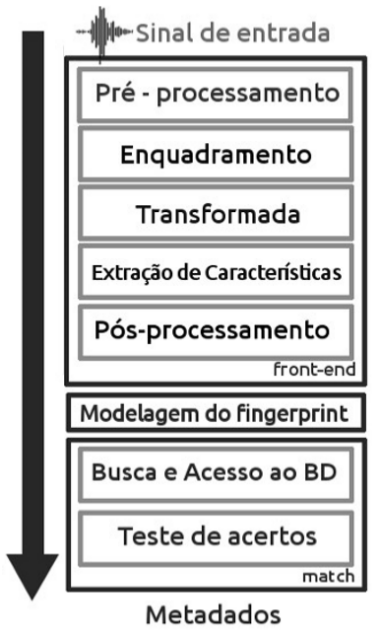
\includegraphics[scale=0.47]{figuras/etapasFinger.png}
   \\Fonte: \cite{carreira2015}.
\end{figure}

No processo de extração do \textit{fingerprint}, chamado de \textit{frontend}, há uma sequência de métodos relevantes até a criação de fato do \textit{fingerprint}. Segundo \citeonline{cano2005}, o primeiro passo é o pré-processamento, onde o som é digitalizado (se necessário) e convertido em um formato genérico, por exemplo, para o formato de 16 bits PCM\footnote{\textit{Pulse Code Modulation}: método usado para representação digital de sinais analógicos.}.

O enquadramento adapta a amostragem convertida para o que será utilizado e \citeonline{cano2005} o definem que:

\begin{citacao}
[...]o sinal é dividido em quadros de um tamanho comparável à velocidade de variação dos eventos acústicos subjacentes. O número de quadros calculados por segundo é chamado de taxa de quadros. Uma função de janela cônica é aplicada a cada bloco para minimizar as descontinuidades no início e no final. A sobreposição deve ser aplicada para garantir robustez ao deslocamento (ou seja, quando os dados de entrada não estão perfeitamente alinhados com a gravação usada para gerar a \textit{fingerprint}) \cite{cano2005}.
\end{citacao}

Em seguida, precisa-se ter o áudio no domínio da frequência \cite{bunnell1996a}. Assim, transformações adicionais são aplicadas que convertem esses sinais em função da frequência, para que o algoritmo de reconhecimento possa realizar uma melhor classificação dentro das características desejadas \cite{santos2011}.

\citeonline{cano2005} citam algoritmos de Transformadas para facilitar a compressão eficiente, a remoção de ruídos e o processamento subsequente:

\begin{itemize}
    \item Transformada de Karhunen-Loève
    \item Tranformada Rápida de Fourier
    \item Transformada de Walsh-Hadamard
    \item \textit{Modulated Complex Lapped Transform (MCLT)}
    \item Transformada Wavelet
\end{itemize}

\citeonline{santos2011} cita um algoritmo prático conhecido como o \textit{espectro do produto harmônico}, ou HPS. Esse algoritmo parte do princípio que o espectro da janela de um sinal de áudio é formado por picos de energia situados na fundamental e na série harmônica da nota. O algoritmo é ilustrado na Figura \ref{fig:hps}, e consiste em multiplicar o espectro do sinal, obtido a partir do algoritmo da Trasformada, por versões comprimidas do próprio espectro. A compressão é realizada reduzindo a amostragem do espectro original por fatores inteiros.

\begin{figure}[!htb]
   \centering
   \caption{Processo da Técnica HPS}\label{fig:hps} 
   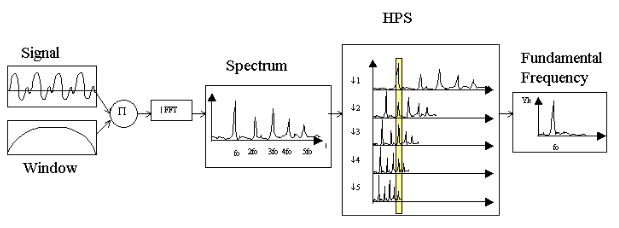
\includegraphics[scale=0.62]{figuras/hps.png}
   \\Fonte: \cite{santos2011}.
\end{figure}

Na extração de características os dados obtidos pela transformada serão novamente transformados com o objetivo de reduzir a dimensionalidade e, ao mesmo tempo, aumentar a invariância às distorções do som para gerar os vetores acústicos finais.

A maioria dos recursos descritos até agora são medições absolutas. E para melhor caracterizar variações temporais no sinal, no pós-processamento, derivadas de tempo de ordem mais alta são adicionadas ao modelo de sinal \cite{cano2005}, conforme mostrado na Figura \ref{fig:extCaract}.

\begin{figure}[!htb]
   \centering
   \caption{Processo de extração de características}\label{fig:extCaract} 
   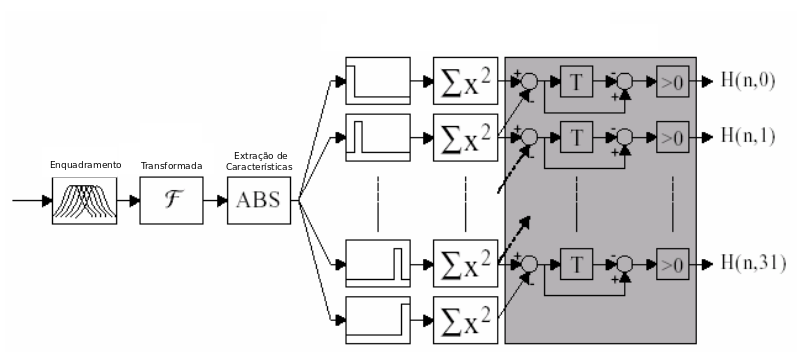
\includegraphics[scale=0.47]{figuras/extCaract.png}
   \\Fonte: \cite{haitsma2002}, editado.
\end{figure}

A modelagem de \textit{fingerprint} geralmente recebe uma sequência de vetores de características calculadas quadro a quadro. E as caracterísitcas escolhidas para montar o modelo de \textit{fingerprint} influenciam a forma como o algoritmo irá tratar futuramente a busca dessas características para comparação. Os modelos podem ser consultados em \cite{cano2005} e \cite{haitsma2002}. Uma forma compacta de \textit{fingerprint} é obtida, e assim, juntamente com informações sobre o formato de áudio original, é enviada para um servidor para identificação, como podemos ver na Figura \ref{fig:identAudio}.

\begin{figure}[!htb]
   \centering
   \caption{Modelagem da identificação de áudio}\label{fig:identAudio} 
   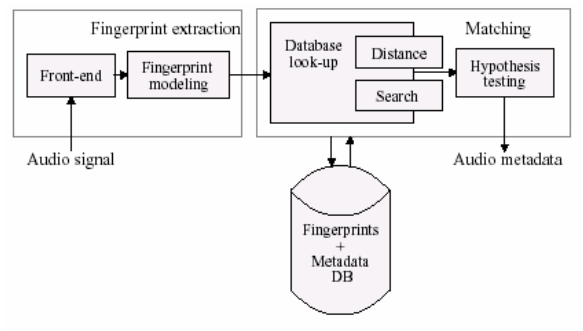
\includegraphics[scale=0.62]{figuras/etapasFinger2.png}
   \\Fonte: \cite{henriques2003}
\end{figure}

No segundo processo, denominado \textit{match}, podemos encontrar uma grande diversidade de algoritmos para localização, identificação e comparação de \textit{fingerprints}. Conforme mencionado anteriormente, o modelo de \textit{fingerprint} escolhido influencia a forma como o algoritmo irá à busca dessas características para comparação. Encontrar \textit{fingerprints} extraídas em um banco de dados de \textit{fingerprints} não é uma tarefa trivial. Em vez de procurar uma \textit{fingerprint} exata (fácil!), a \textit{fingerprint} mais semelhante precisa ser encontrada \cite{haitsma2002}.

A questão fundamental é como fazer a comparação eficiente do áudio desconhecido contra os possíveis milhões de \textit{fingerprints}. Uma abordagem de força bruta que calcule as semelhanças entre a \textit{fingerprint} da gravação desconhecida e as armazenadas no banco de dados pode ser proibitiva. O tempo para encontrar uma melhor correspondência é proporcional a \({N c(d()) + E}\), onde N é o número de \textit{fingerprints} no repositório e \({c(d())}\) o tempo necessário para uma única semelhança e \({E}\) é responsável por algum tempo extra da CPU \cite{cano2005}.

Alguns algoritmos citados por \citeonline{cano2005} que são utilizados para medir a similaridade do conteúdo contido no modelo de \textit{fingerprint}:

\begin{itemize}
    \item Distância Euclidiana, ou versões modificadas que lidam com sequências de diferentes comprimentos.
    \item Distância Manhattan, onde as sequências do vetor são quantizadas, ou distância Hamming quando a quantização é binária.
    \item K-\textit{Nearest Neighbors} ou K-NN, classificação do vizinho mais próximo usando uma estimativa de entropia cruzada.
    \item \textit{Exponential Pseudo Norm} (EPN), utilizada para distinguir melhor entre valores próximos e distantes.
\end{itemize}

Esses algoritmos podem ser encontrados com mais detalhes na subseção \ref{conteudo}.

%CROSS RECURRENCE PLOT%
\subsubsection{Cross Recurrence Plot}

O trabalho de \citeonline{serra2009} propõe o uso de \textit{Cross Recurrence Plots} (CRP\abreviatura{CRP}{Cross Recurrence Plots}) como métrica de similaridade entre músicas. Antes de definir CRP, é necessário introduzir o conceito de \textit{Recurrence Plot} (RP\abreviatura{RP}{\textit{Recurrence Plot}}). RP é uma ferramenta utilizada para visualizar recorrências com uma série temporal, ou seja, regiões onde a órbita da série passa perto de um estado previamente visitado. Mais especificamente, RP é uma matriz quadrada preenchida com zeros e uns, que indicam se há ou não recorrência, ou seja, se o estado no tempo \({i}\) é similar ao estado do tempo \({j}\) \cite{eckmann1987, alligood1996}. A diagonal principal de um RP é, portanto, composta por uns. CRPs sao construídos da mesma maneira que RPs, mas cada eixo corresponde a uma série temporal diferente e a matriz resultante não é quadrada.

Primeiramente, o algoritmo extrai a característica HPCP \cite{gomez2006} de duas músicas, resultando em séries temporais de \({H = 12}\) variáveis. Dados os vetores HPCP da música \textbf{\({x}\)} e da música \textbf{\({y}\)}, calcula-se a transposição de \textbf{\({y}\)} de modo que ela fique na mesma tonalidade de \textbf{\({x}\)}. A transposição ocorre rotacionando-se o vetor HPCP de \textbf{\({y}\)} em \({k}\) posições por meio da técnica \textit{Optimal Transposition Index}, proposta em \cite{serra2009}.

A seguir, calcula-se o \textit{embedding} das duas músicas em um espaço de fase, isto é, um espaço onde as recorrências do sinal podem ser obtidas. Considere que  HPCP \textbf{\({x}\)} tem \({N_{x}^{*}}\) janelas. O \textit{embedding} de \textbf{\({x}\)} é dado por \({x' = \big\{x_{i}\big\}}\), para \({i = 1, ..., N_{x}, N_{x} = N_{x}^{*} - (m - 1)*\tau}\), em que \({x_{i}}\) é calculado com:
\begin{eqnarray} \label{embedding}
    x_{i} &=& (x_{1,i},x_{1,i+\tau}, \ldots, x_{1,i+(m-1)\tau}, \\
          & & x_{2,i},x_{2,i+\tau}, \ldots, x_{2,i+(m-1)\tau}, \nonumber \\
          & & \vdots \nonumber \\
          & & x_{H,i},x_{H,i+\tau}, \ldots, x_{H,i+(m-1)\tau}) \nonumber
\end{eqnarray}

Os autores estimaram os valores ótimos de \({m}\) e \({\tau}\) para o reconhecimento de músicas \textit{cover} por meio da divisão de uma base de dados em conjunto de treinamento e teste. Os parâmetros encontrados foram \({m = 10}\) e \({\tau = 1}\).

\citeonline{serra2009} utilizam a Equação \ref{crp} para calcular o CRP, em que \({\Theta(\cdot)}\) é a função degrau tipo Heaviside \({(\Theta(v) = 0 \ \textrm{se} \ v < 0 \  e \  \Theta(v) = 1, \ \textrm{caso contrário})}\), \({\epsilon_{i}^{x}}\) e \({\epsilon_{i}^{y}}\) são limiares de distâncias e \({|| \cdot ||}\) é a norma Euclidiana. No artigo, os autores calculam os limiares dinamicamente, de modo que 10\% dos vizinhos de cada entrada sejam considerados semelhantes.
\begin{equation} \label{crp}
    R_{i,j} = \Theta(\epsilon_{i}^{x} - ||\mathbf{x_{i} - y_{j}}||)\Theta(\epsilon_{i}^{y} - ||\mathbf{x_{i} - y_{j}}||)
\end{equation}

Em geral, pares de músicas diferentes não exibem nenhum padrão evidente no CRP e pares de músicas \textit{cover} apresentam estrutura de linhas longas e caso contrário, tais padrões não ocorrem.

Com base no CRP de duas músicas, o trabalho de \citeonline{serra2009} propõe o uso do maior comprimento das diagonais formadas na matriz como métrica de similaridade. A medida \({Q_{max}}\) é definida como o maior comprimento das diagonais na matriz CRP, considerando possíveis variações no tempo da música (que correspondem a curvaturas nos traços) e na melodia (pequenas rupturas). Uma análise detalhada para o cáculo do \({Q_{max}}\) pode ser encontrada em \cite{serra2009}.

A partir da medida \({Q_{max}}\), é possível identificar grupos de música \textit{cover} em uma base de dados. Quanto maior o \({Q_{max}}\) entre duas instâncias, maior a probabilidade de elas serem interpretações diferentes da mesma música. Até hoje, \({Q_{max}}\) é considerado o estado da arte em métricas para identificação de músicas \textit{cover}. Sua principal desvantagem é seu alto custo computacional.

%DYNAMIC TIME WARPING%
\subsubsection{Dynamic Time Warping} \label{dtw}

O \textit{Dynamic Time Warping} (DTW\abreviatura{DTW}{\textit{Dynamic Time Warping}}) \cite{keogh2004} é uma técnica que permite definir uma métrica entre séries temporais, por exemplo, características de áudio. Dadas duas séries \({Q}\) e \({C}\) de tamanhos \({n}\) e \({m}\), respectivamente, cria-se uma matriz \({D}\), \({n\times m}\), onde o elemento \({d_{i,j}}\) é a distância entre o elemento \({q_{i}}\) e \({c_{j}}\).

A partir da matriz \({D}\), o algoritmo procura por um caminho mínimo \({W}\), onde \({w_{k} = (i,j)_{k}}\), que respeite as seguintes condições:

\begin{itemize}
    \item Comece em \({(1,1)}\) e termine em \({(n,m)}\);
    \item Percorra apenas índices adjacentes;
    \item Percorra espaçamentos iguais no tempo.
\end{itemize}

O caminho mínimo é encontrado por meio de um algoritmo de programação dinâmica de complexidade \({O(nm)}\) \cite{keogh2004}. A métrica de dissimilaridade DTW é dada por:
\begin{equation}
    DTW(Q,C) = min\left\{\sqrt{\sum_{k=1}^{K} D[w_{k}]}\right\}
\end{equation}

em que \({K}\) é o tamanho do caminho e \({D[w_{k}]}\) é o valor da entrada \({(i,j)_{k}}\) na matriz \({D}\). A Figura \ref{fig:dtw} ilustra a execução do algoritmo DTW.

\begin{figure}[!htb]
   \centering
   \caption{Execução do algoritmo de DTW. (A) Séries C e Q. (B) Matriz de distâncias. (C) Alinhamento das duas séries com o caminho mínimo.}\label{fig:dtw} 
   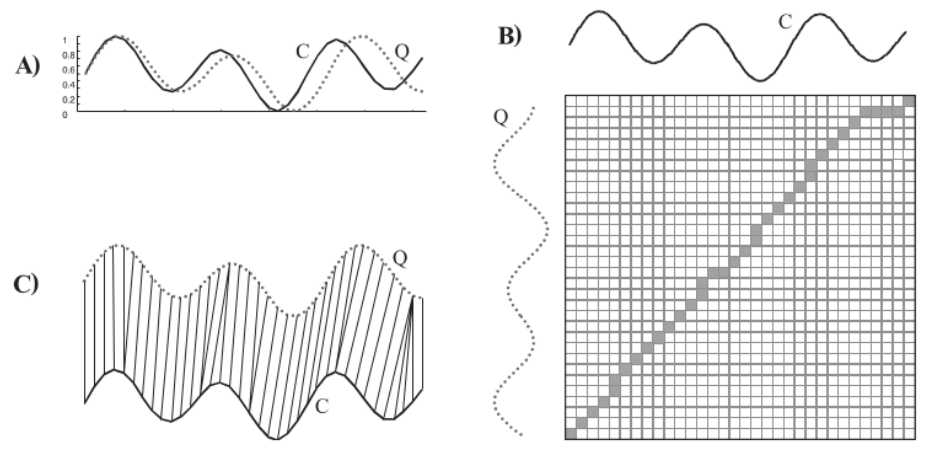
\includegraphics[scale=0.40]{figuras/dtw.png}
   \\Fonte: \cite{keogh2004}.
\end{figure}

Seu uso é inviável em grandes conjuntos de dados. Por este motivo, diversas técnicas de indexação específicas para esse algoritmo foram propostas para a tarefa de busca por similaridade, tais como \textit{lower bound} e \textit{early abandoning}. Com essas técnicas, é possível encontrar os vizinhos mais próximos de uma dada subsequência em uma quantidade massiva de séries temporais. Informações mais detalhadas podem ser consultadas em \cite{mizutani2006}, \cite{kruskal1983} e \cite{juang1991}.

%QUERY BY HUMMING%
\subsubsection{Query by Humming}
A tarefa de busca musical a partir de um trecho de música cantada ou cantarolada pelo usuário passou a ser conhecida na literatura como \textit{query by humming}, ou QBH. É um sistema capaz de reconhecer música pelo \textit{casamento aproximado} de cadeias de caracteres. \citeonline{ghias1995}, autores do projeto, aplicaram o conceito de \textit{contorno melódico}, ou seja, a forma natural como nós percebemos a música. A Figura \ref{fig:qbh} mostra a arquitetura do sistema.

\begin{figure}[!htb]
   \centering
   \caption{Modelagem do Sistema de QBH}\label{fig:qbh} 
   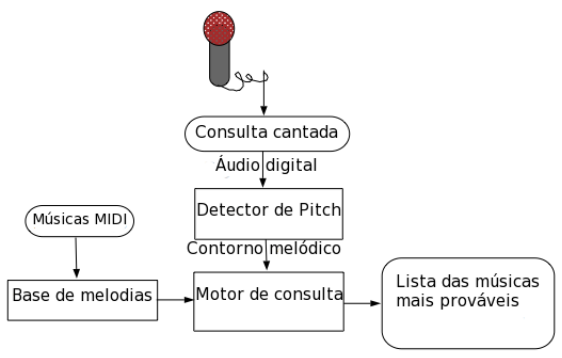
\includegraphics[scale=0.50]{figuras/qbh.png}
   \\Fonte: \cite{santos2011}.
\end{figure}

Segundo \citeonline{santos2011}, existem dois principais interesses em QBH: Primeiramente, permitir ao usuário identificar uma música da qual não conheça (ou lembre de) qualquer metadado associado (autor, álbum, título da música, entre outros). Em segundo, é dispor de uma maneira mais natural para consultar coleções de músicas digitais armazenadas principalente em dispositivos portáteis.

A base de dados de um sistema de QBH é, frequentemente, construída a partir da transposição de músicas MIDI para o formato de representação musical adotado pelo sistema (formatos vistos na seção \ref{formatos}). Para casos em que a técnica de reconhecimento baseia-se em propriedades estatísticas associadas à incerteza do canto, é necessário também estimar os parâmetros do modelo. Para estimá-los, no entanto, precisamos de gravações da mesma música por diferentes usuários. Por este motivo, uma plataforma com este algoritmo estará em constante crescimento e aprendizado.

Capturar o sinal de áudio que codifica uma música cantada por um usuário, seja para construir a base de dados, seja para consultar o sistema por músicas conhecidas, requer atenção quanto ao nível de ruído do ambiente, à taxa de amostragem e à expressão fonética permitida. 

Conforme visto na seção \ref{audioFingerprint}, alguns métodos utilizados no \textit{frontend} para a criação de uma \textit{fingerprint}, também são utilizados para a segmentação e enquadramento do som utilizado pelo algoritmo QBH, deixando a representação musical em função do tempo.

Em seguida, a tarefa executada no sistema QBH é propor ao usuário uma lista de músicas que melhor correspondam à consulta, adotando uma medida de dissimilaridade apropriada entre os arquivos.

A similaridade entre as músicas no repositório e a consulta é calculada por meio do DTW, visto na subseção \ref{dtw}, que o torna particularmente adequado para recuperação em sistemas QBH. Podemos ver o processo na Figura \ref{fig:qbhProcesso}.

\begin{figure}[!htb]
   \centering
   \caption{Sistema de QBH}\label{fig:qbhProcesso} 
   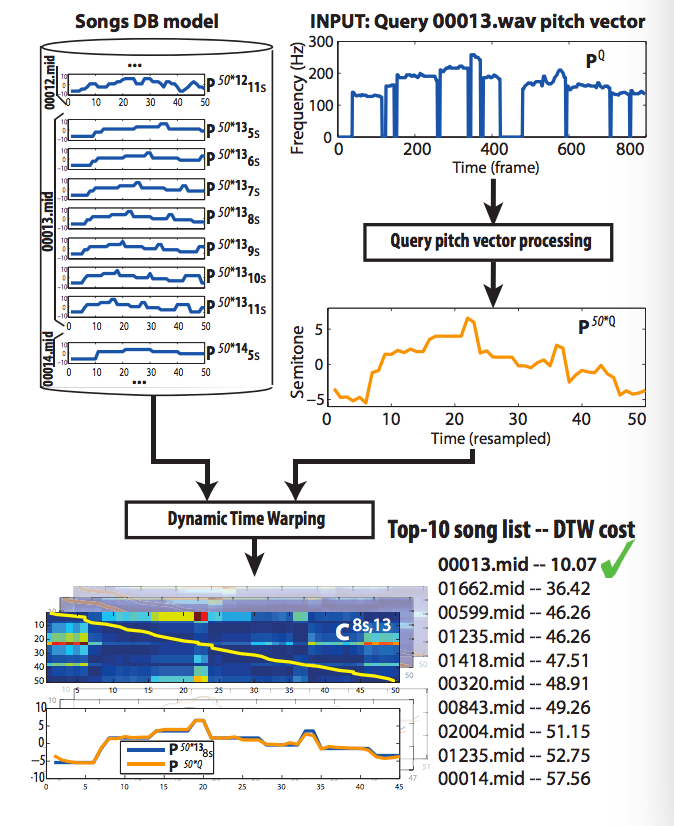
\includegraphics[scale=0.95]{figuras/query_by_humming.png}
   \\Fonte: ACRCloud.
\end{figure}

Desta forma, vários tipos de sistemas QBH foram pesquisados:

\citeonline{wang2008} propuseram o sistema de QBH combinando as distâncias do \textit{earth mover’s distance} (EMD) e do \textit{dynamic time warping} (DTW) baseado na regra de soma ponderada.

\citeonline{ryynanen2008} propuseram o método de extração dos vetores \textit{pitch} através do uso de uma janela de tempo de tamanho fixo e comparando-os por meio do método \textit{locality sensitive hashing} (LSH).

\citeonline{salamon2009} propuseram recuperação em dois estágios para o sistema QBH. No primeiro estágio, o número de candidatos é reduzido através do método de indexação utilizando \textit{ngrams}. Depois, um método de comparação mais sofisticado é aplicado com os candidatos restantes baseado no alinhamento local com funções de custos modificados.

Embora os sistemas atuais de última geração para QBH tenham alcançado um desempenho razoável em casos do mundo real, ainda há muito espaço para a melhoria na indexação de músicas e o método de correspondência do sistema QBH, especialmente em um banco de dados de música na escala da web.

%RECUPERAÇÃO POR CONTEÚDO%
\subsubsection{Recuperação por Conteúdo} \label{conteudo}
As técnicas baseadas em busca por conteúdo utilizam características extraídas automaticamente dos dados complexos para representar e indexar as informações embutidas nesses dados, como artista, álbum e título da música. Cada características é usualmente um valor ou um conjunto de valores numéricos e o conjunto de características extraídas é chamado vetor de características. Nos sistemas de recuperação por conteúdo, as operações de comparação entre dados complexos utilizam os vetores de características para medir a similaridade do conteúdo presente nos dados que eles representam.

\begin{enumerate}
    \item Distância Euclidiana ou Distância Métrica
    
    Frequentemente utilizada com uma medida de distância entre dois pontos em planos n-dimensionais (ver Figura \ref{fig:euclidiana}), que pode ser provada pela aplicação repetida do teorema de Pitágoras. À medida que o número de dimensões aumenta, o tempo de cálculo também aumenta.
    
    A distância euclidiana entre os pontos \({P=(p_{1},p_{2},\ldots,p_{n})}\) e \({Q=(q_{1},q_{2},\ldots, q_{n})}\) num espaço euclidiano n-dimensional, é expressa na Equação \ref{euclidiana}.
    
    \begin{equation} \label{euclidiana}
        \sqrt {(p_{1}-q_{1})^{2}+(p_{2}-q_{2})^{2}+\ldots +(p_{n}-q_{n})^{2}}=\sqrt {\sum _{i=1}^{n}(p_{i}-q_{i})^{2}}
    \end{equation}
    
    \begin{figure}[!htb]
       \centering
       \caption{Distância Euclidiana entre os pontos A e B}\label{fig:euclidiana} 
       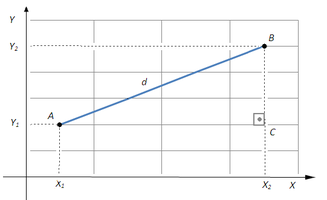
\includegraphics[scale=0.85]{figuras/euclidiana.png}
       \\Fonte: Internet.
    \end{figure}
    
    \item Distância de Manhattan
    
    É uma medida de distância entre dois pontos em um espaço euclidiano com um sistema de cartesiano de coordenadas fixas (ver Figura \ref{fig:manhattan}). É a soma dos comprimentos da projeção da linha que une os pontos com os eixos das coordenadas.
    
    Em um plano que contém os pontos \({P_{1}}\) e \({P_{2}}\), com as coordenadas \({(x_{1},y_{1})}\) e \({(x_{2},y_{2})}\) respectivamente, é definido através da Equação \ref{manhattan}.
    
    \begin{equation} \label{manhattan}
        \left|x_{1}-x_{2}\right|+\left|y_{1}-y_{2}\right|
    \end{equation}
    
    \begin{figure}[!htb]
       \centering
       \caption{Distância de Manhattan (linhas roxa, verde e vermelha)}\label{fig:manhattan} 
       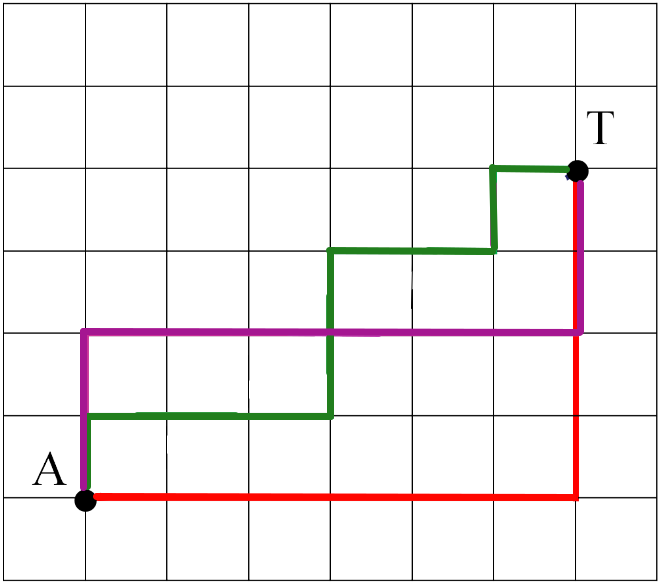
\includegraphics[scale=0.32]{figuras/manhattan.png}
       \\Fonte: Internet.
    \end{figure}

    \item Distância de Minkowski
    
    Esta distância é a generalização das duas distâncias: Euclidiana e Manhattan (ver Figura \ref{fig:minkowski}), que é definida pela Equação \ref{minkowski}.
    
    \begin{equation} \label{minkowski}
        d(x,y)=(\left|x_{1}-y_{1}\right|_{q} + \left|x_{2}-y_{2}\right|_{q} + \cdots + \left|x_{n}-y_{n}\right|_{q})^{\frac{1}{q}}\textrm{, onde q} \in N
    \end{equation}
    
    Quando \({q=1}\), esta distância representa a distância de Manhattan e quando \({q=2}\), a distância Euclidiana.
    
    \begin{figure}[!htb]
       \centering
       \caption{Distância de Manhattan (linhas rosa, verde e vermelha) e Distância Euclidiana (linha azul)}\label{fig:minkowski} 
       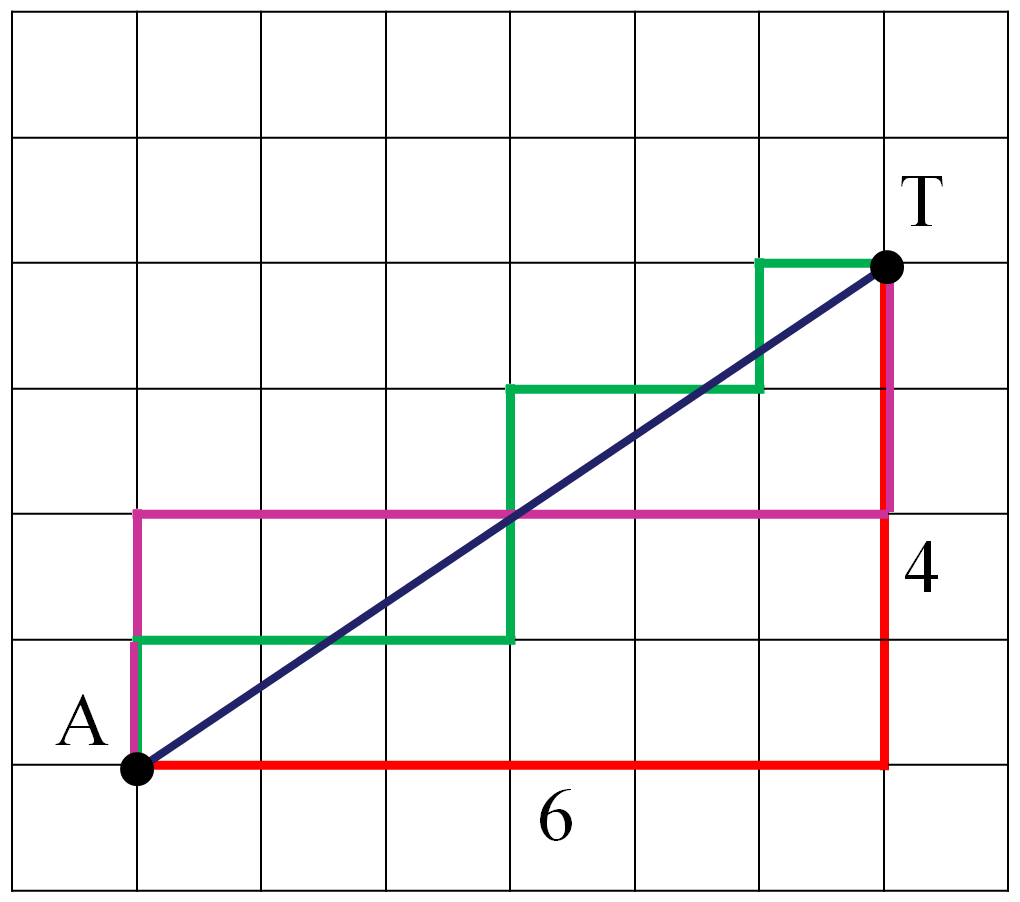
\includegraphics[scale=0.20]{figuras/minkowski.png}
       \\Fonte: Internet.
    \end{figure}

    \item K-\textit{Nearest Neighbors} ou K-NN
    
    É um classificador onde o aprendizado é baseado na analogia. O conjunto de treinamento é formado por vetores n-dimensionais e cada elemento deste conjunto representa um ponto no espaço n-dimensional.
    
    Para determinar a classe de um elemento que não pertença ao conjunto de treinamento, o classificador procura K elementos do conjunto de treinamento que estejam mais próximos deste elemento desconhecido, ou seja, que tenham a menor distância.
    
    Estes K elementos são chamados de \textit{K-Nearest Neighbors} (K-vizinhos mais próximos, traduzido). Verifica-se quais são as classes desses K vizinhos e a classe mais frequente será atribuída à classe do elemento desconhecido. O número de K-vizinhos é um parâmetro livre controlado pelo usuário com o objetivo de obter uma melhor classificação (ver Figura \ref{fig:knn}).
    
    As métricas mais comuns utilizadas para o cálculo da distância são: Distância Euclidiana, Distância de Manhattan e Distância de Minkowski.
    
    Este processo de classificação pode ser computacionalmente exaustivo se considerado um conjunto com muitos dados, mas para determinadas aplicações, no entanto, o processo é bem aceitável \cite{knn}.
    
    \begin{figure}[!htb]
       \centering
       \caption{K-Nearest Neighbors}\label{fig:knn} 
       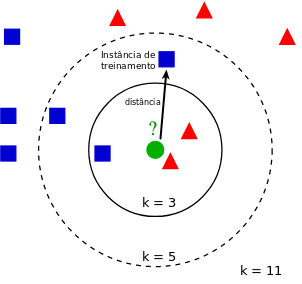
\includegraphics[scale=0.80]{figuras/knn.png}
       \\Fonte: Internet, editado.
    \end{figure}

    \item \textit{Exponential Pseudo Norm} (EPN)
    
    A distribuição exponencial surge em conexão com os processos de Poisson. Um processo de Poisson é aquele que exibe um padrão de chegada aleatória no seguinte sentido:
    \begin{enumerate}
        \item Para um pequeno intervalo de tempo \({\Delta t}\), a probabilidade de uma chegada durante \({\Delta t}\) é \({\lambda \Delta t}\), onde \({\lambda}\) = a taxa média de chegada;
        \item A probabilidade de mais de uma chegada durante \({\Delta t}\) é insignificante;
        \item O tempo e chegada são independentes uns dos outros.
    \end{enumerate}
    
    Este é um tipo de processo "estocástico", no qual os eventos ocorrem de forma aleatória. Sob estas suposições, pode-se mostrar que a \textit{Probability Density Function} (pdf) para a distribuição dos tempos entre chegadas é definida através da Equação \ref{distribuicaoTempo}.
    
    \begin{equation} \label{distribuicaoTempo}
        f(x) = \lambda e^{-\lambda ,x}
    \end{equation}
    
    Sendo que o pdf é dada pela função \({f \colon R \rightarrow [0,1]}\) tal que \({\int_{R}f(x)dx = 1}\), e a função de distribuição para o pdf é definida através da Equação \ref{definitionFunction}.
    
    \begin{equation} \label{definitionFunction}
        F(x) = \int_{-\infty}^{x}f(z)dz
    \end{equation}
    
    Desta forma, se puder ser mostrado que o número de chegadas durante um intervalo é distribuído por Poisson, então os tempos entre chegadas são distribuídos exponencialmente, sendo que a taxa média de chegada é dada por \({\lambda}\) e o tempo médio entre chegadas é dado por \({1/\lambda}\). A distribuição de Poisson é uma distribuição discreta intimamente relacionada à distribuição binomial.
    
    Este algoritmo é apresentado com mais detalhes no trabalho do autor \cite{winton2011}.
    
    \item \textit{Longest Common Subsequence} (LCS)
    
    É a maior subsequência de caracteres comuns que há entre dois objetos (ver Figura \ref{fig:lcs}).
    
    Dada duas sequências \({X}\) e \({Y}\) de comprimento \({m}\) e \({n}\), respectivamente, onde \({}\)
    \({X = \left\{X_{1}, X_{2}, \ldots, X_{m} \right\} }\) e \({Y=\left\{Y_{1}, Y_{2}, \ldots, Y_{n} \right\}}\) definimos \({LCS(X,Y)}\) como a máxima subsequência comum entre \({X}\) e \({Y}\). A equação de recorrência para o cálculo de \({LCS(X,Y)}\) pode ser deduzida a partir de duas propriedades:
    
    \begin{enumerate}
        \item Se \({X_{1}=Y_{1}}\), então \({LCS(X,Y)}\) é a concatenação de \({X_{1}}\) com \({LCS(X_{2:m},Y_{2:n})}\).
        \item Se \({X_{1} \not= Y_{1}}\), então \({LCS(X,Y)=max(LCS(X_{2:m},Y), LCS(X,Y_{2:n}))}\).
    \end{enumerate}

    Estas propriedades constituem a sub-estrutura ótima para a resolução continuada do primeiro caractere de cada string com a aplicação recursiva dessas mesmas propriedades ao sufixo remanescente. As mesmas propriedades são válidas quando as strings são analisadas do fim para o começo, resolvendo o último caractere e aplicando a recursão ao prefixo remanescente:
    
    \begin{enumerate}
        \item Se \({X_{m}=Y_{n}}\), então \({LCS(X,Y)}\) é a concatenação de \({LCS(X_{1:m-1},Y_{1:n-1})}\) com \({X_{m}}\).
        \item Se \({X_{m} \not= Y_{n}}\), então \({LCS(X,Y)=max(LCS(X_{1:m-1},Y), LCS(X,Y_{1:n-1}))}\).
    \end{enumerate}
    
    As definições matemáticas das recursões por sufixo e prefixo são respectivamente apresentadas nas Equações \ref{sufixo} e \ref{prefixo}:
    
    \begin{equation} \label{sufixo}
        LCS(X,Y) =
            \begin{cases}
            \emptyset & \quad \textrm{se } m=0 | n=0\\
            X_{1}+LCS(X_{2:m},Y_{2:n})  & \quad \textrm{se } X_{1}=Y_{1}\\
            max(LCS(X,Y_{2:n}),LCS(X_{2:m},Y)) & \quad \textrm{se } X_{1}\not=Y_{1}
            \end{cases}
    \end{equation}
    
    \begin{equation} \label{prefixo}
        LCS(X,Y) =
            \begin{cases}
            \emptyset & \quad \textrm{se } m=0 | n=0\\
            LCS(X_{1:m-1},Y_{1:n-1})+X_{m}  & \quad \textrm{se } X_{1}=Y_{1}\\
            max(LCS(X_{1:m-1},Y),LCS(X,Y_{1:n-1})) & \quad \textrm{se } X_{1}\not=Y_{1}
            \end{cases}
    \end{equation}
    
    \begin{figure}[!htb]
       \centering
       \caption{Longest Common Subsequence}\label{fig:lcs} 
       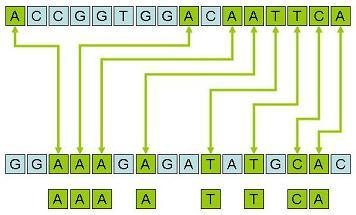
\includegraphics[scale=1.0]{figuras/lcs.jpg}
       \\Fonte: Internet.
    \end{figure}
    
    Este algoritmo é apresentado com mais detalhes no trabalho dos autores \citeonline{cormen2009}.

\end{enumerate}

%INDEXAÇÃO%
\subsubsection{Indexação}
Indexação é um processo pelo qual as características extraídas dos dados complexos (como artista, álbum e título da música) são armazenados em uma estrutura de índice para facilitar e acelerar a tarefa de busca dos dados musicais.

Na literatura podem ser encontradas variadas formas de indexação para dados musicais. Portanto, o objetivo nesta subseção é descrever de forma genérica como funcionam os métodos de indexação e citar os mais conhecidos para indexação de dados musicais.

Estruturas de indexação são normalmente fornecidas pelos SGBD. Embora essas estruturas de indexação sejam suficientes para suprir as necessidades dos usuários de aplicações que lidam com dados convencionais, elas não são adequadas para os sistemas de recuperação de dados complexos, que lidam com dados que apresentam alta dimensionalidade e não apresentam relação de ordem \cite{barioni2006}.

A idéia básica dessas estruturas consiste na escolha de um objeto arbitrário central e na aplicação de uma função de distância para dividir os demais objetos em vários subconjuntos. Dessa maneira, a estrutura de indexação é construída executando-se esse mesmo procedimento, recursivamente, para cada subconjunto não vazio.

Os métodos de indexação mais conhecidos na literatura e aplicados à indexação de dados musicais são a \textit{VP-tree} (\textit{Vantage Point tree}) \cite{yanilos1993}, a \textit{MVP-tree} (\textit{Multi-Vantage Point tree}) \cite{bozkaya1997}, a GNAT (\textit{Geometric Near-neighbor Access Tree}) \cite{brin1995}, a \textit{M-tree} \cite{ciaccia1997}, a \textit{Slim-tree}, \textit{Família-Omni} e a \textit{DBM-tree} \cite{traina2000, filho2001, vieira2004}, a \textit{n-grams} \cite{downie1999} e o \textit{Vantage Indexing Method} \cite{typke2003}.
